\appendices
\section{Exact Ship Model}
\label{appendix:exact_model}

The model used in the simulations is, in continuous time,
\begin{equation}
    \dot{x}(t) = A_c x(t) + B_c u(t) + E_{d,c} d(t) + E_{f,c} f(t),
\end{equation}
\begin{equation}
    y(t) = C_c x(t) + D_c u(t) + G_{d,c} d(t) + G_{f,c} f(t),
\end{equation}
with
\begin{equation}
    A_c = \begin{bmatrix}
        b\eta_1 & 0 \\
        1 & 0
    \end{bmatrix},
    \quad
    B_c = \begin{bmatrix}
        b \\
        0
    \end{bmatrix},
    \quad
    E_{d,c} = \begin{bmatrix}
        0 \\
        1
    \end{bmatrix},
\end{equation}
\begin{equation}
    E_{f,c} = \mathbf{0}, \quad \text{and} \quad \begin{cases}
        b = 2.2\\
        \eta_1 = -10
    \end{cases}.
\end{equation}

The output equation matrices are
\begin{equation}
    C_c = \begin{bmatrix}
        1 & 0 \\
        0 & 1
    \end{bmatrix},
    \quad
    D_c = 0,
\end{equation}
\begin{equation}
    G_{d,c} = \begin{bmatrix}
        1 \\
        0
    \end{bmatrix},
    \quad
    G_{f,c} = \begin{bmatrix}
        1 & 0 \\
        0 & 1
    \end{bmatrix}.
\end{equation}

The discrete-time model in (\ref{eq:ss_model}) is finally obtained using a ZOH discretization with sampling time $T_s = 0.2$ seconds.

\section{Three-Phased signal Model}
\label{appendix:three_phased_model}

Fig. \ref{fig:data} shows the signal in a case no fault is applied. Knowing the sampling period $T_s = 1$ms, the frequency of the signal is computed by
\begin{equation}
    \omega_{\text{exc}} = \frac{2 \pi}{50  T_s}
\end{equation}
because there are $50$ measurements per period.

\begin{figure}[htbp]
    \centering
    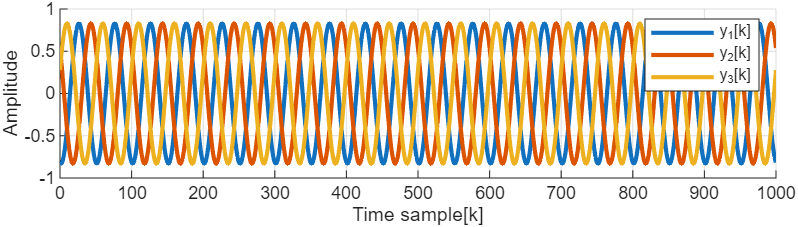
\includegraphics[width=0.48\textwidth]{../Matlab/ObserverMethods/Data.png}
    \caption{Three-phased signal measured by 3 (faultless) sensors.}
    \label{fig:data}
\end{figure}

The continuous-time state space model of this system (which has no input) is given by
\begin{equation}
    \mathbf{\dot{x}} = \begin{bmatrix}
        0 & \omega_{\text{exc}}\\
        -\omega_{\text{exc}} & 0
    \end{bmatrix} \mathbf{x}.
\end{equation}
Because there is an offset between the three phases, the output relationship is expressed as follows, where $\mathbf{f}$ is the fault vector:
\begin{equation}
    \mathbf{y} = \begin{bmatrix}
        \cos(0) & \sin(0)\\
        \cos(\frac{-2 \pi}{3}) & \sin(\frac{-2 \pi}{3}) \\
        \cos(\frac{2 \pi}{3}) & \sin(\frac{2 \pi}{3}) \\
    \end{bmatrix} \mathbf{x} + \mathbf{f}.
\end{equation}

This continuous-time model is then discretized using the ZOH with the known sampling frequency.

